\chapter{Rozbor řešené problematiky}
\label{sec:RozborReseneProblematiky}

Počítače jsou nedílnou součástí dnešního života. Jejich využítí je prakticky neodmyslitelné ať se jedná o superpočítače pro složité výpočty, servery, klasické stolní počítače nebo o jednoúčelové počítače. Proto je důležíté testovat a sledovat výkon těchto počítačů, aby jejich využítí bylo co nejvíce efektivní. Zároveň lze tímto zjistit, zda je daný počítač dostatečný na vykonávání dané úlohy. Tato kapitola obsahuje přehled základních informací týkajících se počítačového výkonu, jeho měření a testování, a přehledu nástrojů.


\section{Počítačový výkon}
Počítačový výkon je účinnost daného systému neboli jak dobře funguje, když se vezmou v úvahu všechny možné aspekty.
Hodnocení výkonu počítače je definováno jako proces při kterém se posuzují zdroje a výstupy počítače, aby se zjistilo,
jestli systém funguje na optimální úrovni.

Počítačové vyhodnocování je složitý proces. Při vyhodnocování výkonu počítače se k určení využívá řada aspektů.
\paragraph{Hlavní aspekty}\cite{MetricsToday}
\begin{itemize}[noitemsep]
    \item{škálovatelnost}
    \item{stabilita}
    \item{schopnost reagovat}
    \item{rychlost}
    \item{dostupnost}
    \item{propustnost}
    \item{doba odezvy}
    \item{spolehlivost}
    \item{provozuschopnost}
\end{itemize}

Ke zjištění těchto aspektů se využívají speciálně navržené programy, které posuzují relativní výkon daného objektu obvykle spuštěním řady testů.
Tento proces se nazývá benchmark. Není jednoduché vytvořit měřítka pro hodnocení výkonu počítaču, protože technologické vlastnosti se stále vývíjí a obměňují.
Toto znamené, že benchmark počítačů musí být také neustále vyvíjen a aktualizován.

\iffalse
https://study.com/academy/lesson/computer-performance-evaluation-definition-challenges-parameters.html
\fi



\section{Meření výkonu}

Měřící technika hodnocení výkonu počítačů je považována za nejvíce důvěryhodnou, ale zároveň za nejvíce drahou. Může být implementována na skutečný systém nebo na prototypovou verzi systému, který bude sestaven. Měření výkonu systému zahrnuje monitorování systému zatím co je v pracovní zátěži nebo je nad ním spuštěna sada testovacích aplikací.

Základem je, aby člověk, který bude měřit, rozuměl těmto hlavním konceptům než začne měřit:
\begin{itemize}[noitemsep]
    \item{systémové aplikace}
    \item{metriky výkonu, které budou měřeny}
    \item{hardwarové vybavení systému}
    \item{zátěž pro skutečnou aplikace}
    \item{způsob prezentace výsledků měření}
\end{itemize}

\section{Cíle měření výkonu}

Cíle měření výkonu závisí na zájmu, aplikaci(systému), zručnosti a znalosti člověka, který bude měřit. Nicméně základní cíle jsou vypsány níže.

\subsection*{Porovnání alternativních návrhů systému}

Cílem je porovnat výkony různých systémů nebo návrhů komponent pro konkrétní aplikaci. Například výběr optimálního počtu procesorů v paralelním systému, velikost a počet disků nebo výběr správného operačního systému. Cílem, v tomto případě, je najít nejlepší možné řešení konfigurace v uvažovaných operačních prostředcích.

\subsection*{Pořizování}

V tomto případě je hlavním cílem najít nejefektivnější systém pro danou aplikaci. Je nezbytné zvážit přínos dražší verze daného systému, který poskytne jen malé zvýšení výkonu v porovnání s levnějším systémem.

\subsection*{Plánování kapacity}

Toto je speciální a zajímavé pro správce zařízení pro zpracování dat a systémové administrátory. Cílem je se ujistit, zda budou k dispozici dostatečné zdroje pro splnění budoucích požadavků způsobem, který bude efektivní a neohrozí výkon.

\subsection*{Vylepšení dosavadního systému}

Cílem je najít nejepší sadu parametrů, která poskytne nejlepší výkon celého systému. Například použití rychlejšího disku nebo zvýšení velikosti vyrovnávací paměti může vést ke zvýšení výkonu.

\subsection*{Odladění výkonu}

Někdy může nastat situace, kdy některé aplikace nebo systém fungují, ale pracují pomalu. Je tedy nezbytné analyzovat výkon a zjistit, proč program nebo systém nesplňuje dané očekávání. Pokud je příčína odhalena, může být vyřešena.

\subsection*{Ukázat, co systém dokáže}

Cílem je ukázat uživatelům, co systém skutečne zvládne a dokáže. Toto je nezbytné pro vývoj nových počítačových komponentů jako jsou například procesory.

\section{Metriky k měření}

Před každým měřením by mělo být jasně dáno jaké metriky budeme měřit a jakým způsobem se to bude vykonávat. Pokud metriky ani způsob nebude
stanoven, tak je měření ztrátou času. Ověření těchto metrik se poté provádí testováním. Svoji důležitou roli hraje také složitost tesovaného
softwaru. Mezi základní metriky k měření výkonu systému jsou:

\subsection*{Doba spuštění a doba načítání}

Každý software vyžaduje nějaký čas k jeho načtení a zahájení provozu. Koncový uživatelé během této doby obvykle vidí animovaný kurzor nebo
načítání obrazovky. Složité programy mohou vyžadovat nastavení a konfiguraci než uživatele pustí do práce. Software například kontroluje
závislost s jiným softwarem nebo existenci potřebných souborů. Toto zvyšuje jeho dobu načítání. Doba načítání by proto měla být co nejkratší.

\subsection*{Doba odezvy nebo latence}

Doba odezvy označováná jako latence je doba prodlevy mezi okamžikem, kdy uživatel zadá vstup, a okamžikem, kdy daný software na základě tohoto vstupu reaguje.
V ideálním připadě by tato doba měla být pro uživatele neposřehnutelná. Tato doba také může záviset na hardwaru nebo na rychlosti připojení k internetu.

\subsection*{Omezené zatížení nebo špatná škálovatelnost}

Aplikace by měly obsluhovat omezený počet zařízení nebo uživatelů bez snížení výkonu softwaru. Škálovatelnost pomáhá zajistit, aby aplikace měla prostředky pro podporu očekávaného počtu uživatelů.
Testování výkonu hodnotí software při různých podmínkách zátěže. Nedostatečné zdroje, jako je nedostatečný výpočetní výkon, mohou způsobit špatnou škálovatelnost.
Mnoho problémů se škálovatelností může vyplývát ze špatné architektury aplikací. Každá aplikace by měla být naprogramovaná tak, aby se dala případně v budoucnu škálovat.

\subsection*{Uzká místa}

Každá aplikace přistupuje k omezeným zdrojům, jako třeba výpočetní výkon, šířka pásma, propustnost sítě, kapacita diskového ůložiště a vstupy/výstupy
a služby operačního systému. Úzká místa(angl. bottlenecks) jsou nedostatky zdrojů, ke kterým dochází pokud software není vhodně navržen nebo pokud systém pro danou aplikaci není dostačující.

\subsection*{Propustnost}

Propustnost je počet jednotek dat, které systém zpracuje za určitou dobu.

\iffalse
\subsection*{Spolehlivost, dostupnost, provozuschopnost}

RAS označuje schopnost softwaru trvale plnit své specifikace; jak dlouho funguje vzhledem k očekávanému množství; a jak snadno se dá opravit nebo udržovat.


najit nejaky zdroj k propustnisti
https://searchsoftwarequality.techtarget.com/answer/Required-prerequisites-for-performance-testing
\fi

\section{Typy událostí}

V měřící technikách se často měří jiné vykonnostní metriky. Toto závisí na aplikace nebo systém, který bude testován. Z pohledu typu události se metriky kategorizují do následujících skupin.

\subsection*{Metriky počtu vyvolaných událostí}

Tato třída zahrnuje metriky, které jednodušee počítají počet vykonání nějaké konkrétní události. Například počet paketu, které jsou zahozeny nebo počet vynechání vyrovnávací paměti.

\subsection*{Profily}

Profily v počítačových systémech představují souhrnou metriku pro charakterizaci celého systému nebo chování aplikace. Například stupeň paralelismu představuje celkový počet aktivních procesorů v paralelním počítačovém systému v okamžiku vykonávání konkrétního aplikace.

\subsection*{Metriky pomocných událostí}

Pomocí pomocných metrik se zaznamenávají hodnoty sekundárních systémových parametrů, když se vykoná konkrétní událost.

\section{Strategie měření}

O strategii, pro sledování metrik výkonu, je možné rozhodnout na základě použíté výše uvedené klasifikace typu událostí. Hlavní strategie jsou následující.

\subsection*{Událostmi řízená strategie}

Údálostmi řížená strategie zaznamenává informace potřebné pro vypočítání nějaké metriky, kdykoliv nastane událost, která je spojená s danou metrikou. Například takovou metrikou může být počet vynechání vyrovnávací paměti. Toto číslo by mělo být aktualizováno vždy, když nastane příslušná událost. Po ukončení měření počítadlo vrátí svůj obsah. Výhoda této strategie je, že režie potřebná k monitorování událostí, které jsou s tím spojené, se utrácí pouze pokud k události dojde. Tato vlastnost je však nevýhodná, pokud se události vyskytují často.

\subsection*{Sledovací strategie}

Tato stategie se opírá o záznam sledování více událostí než pouze jediné. Tato strategie vyžaduje více uložného prostoru ve srovnání s událostmi řízenou strategii.

\subsection*{Nepřímá strategie}

Toto schéma se využívá při měření výkonu, které nelze měřit přímo. V takovém případě je důležité najít metriku ze které lze dané požadované metriky vyvodit.

\subsection*{Vzorkovací strategie}

Vzorkovací strategie zaznamenává potřebné stavy systému ke zjištění metrik, které byly zvolené. Z tohoto vyplývá, že vzorkovací frekvence určuje celkovou režii a kvalitu měření. Vzorkovací frekvence se určuje podle požadovaných událostí.

\iffalse
https://www.cin.ufpe.br/~rmfl/ADS_MaterialDidatico/PDFs/simulacaoTransiente/FUNDAMENTALS%20OF%20PERFORMANCE%20EVALUATION%20OF%20COMPUTER%20AND%20TELECOMMUNICATION%20SYSTEMS.pdf

https://books.google.cz/books?hl=cs&lr=&id=BPJgCL1LnHgC&oi=fnd&pg=PR7&dq=computer+performance+evaluation&ots=VplZBicCmv&sig=vl6x2R5wa0izwenpyXAQs6n8vrA&redir_esc=y#v=onepage&q=computer%20performance%20evaluation&f=false
flops



\section{Metody zjišťování výkonu}

Vyhodnocování výkonu počítačů je důležitou technologii pro výzkum v oblasti počítačů. Neustálý vývoj počítačů dělá tento úkol stále složitější.
Obecný problém rozvoje efektivní vyhodnocovací techniky lze vyjádřit jako hledání nejlepšího kompromisu mezi přesností a rychlostí. Tento kompromis závisí na
použití vyhodnocovací metody. Správná efektivita může vést ke snížení nákladů při tvorbě systému pro běh aplikace.

\fi

\section{Testování}

Vzhledem k velkému potenciálu hrozeb v souvislosti s výkonem softwaru, mohou různé testy zaměřené na výkon vyhodnitit specifické chování softwaru. Mezi důležité typy testů patří:

\subsection*{Zátěžové testy}

Tento typ testů obecně měří pohyb dat, také nazývaný jako propustnost. Zátěživý test pomáhá ověřit zda daný software funguje správně za typických podmínek. Cílem zátěžového testování je zajistit,
aby klíčové metriky výkonu, jako propustnost dat za sekundu nebo přístup disku za sekundu, zůstaly přijatelné, když se připojí více zařízení nebo více uživatelů. Pokud testování významně
ovlivňuje metriky výkonu, tak je to signál k úpravě softwaru. Případně zjištění maximálního limitu softwaru.

\subsection*{Odolnostní testy}

Odolnostní testy jsou charakteristické tím, že se provádí po delčí dobu. Jejich cílem je ověřit, jestli se výkonnostní charakteristiky softwaru v průběhu provádění nemění. Odolnostní testy
zachycují nedostatky jako je nedostatečná paměť. Při krátkém testování by se tento problém nemusel vůbec objevit.

\subsection*{Spike testy}

Spike testy simulují náhle změny uživatelské zátěže za účelem měření odezvy softwaru.

\subsection*{Závislostní testy}

Software zřídka funguje sám o sobě. Většinou spoléha na jiné aplikace nebo případně na databázi. Testy závislosti vyhodnocují výkon softwaru při zátěži, ale vztahují se na závislosti, nikoliv
jen na software.

\iffalse
https://searchsoftwarequality.techtarget.com/answer/Required-prerequisites-for-performance-testing
\fi



\iffalse
\subsection{Existující řešení}
\fi



\section{Nástroje}

Tato sekce slouží jako přehled nástrojů, které byly využíté při tvorbě této bakalářské práce.

\subsection{Berkeley Packet Filter}
\label{sec:BPF}

Berkeley Packet Filter\cite{BPFPerformanceTools} nebo také BPF je technologie, která byla původně vyvinuta jako nástroj na zachytávání paketů. Poté zaznamenala zásadní změny a byla zahrnuta do linuxového jádra. Takto se z BPF stal univerzální nástroj pro spouštění, který lze využít pro mnoho věcí včetně vytváření nástrojů na analyzování výkonu.
Rozšíří schopnosti jádra bez nutnosti měnit zdrojový kód jádra, díky spouštění mini programů připojených na \hyperref[sec:SledovaniUdalosti]{událostech}.

BPF je flexibilní a efektivní technologie složená z instrukční sady a pomocných funkcí. BPF instrukce nejprve prochází ověřovatelem, který zajistí bezpečnost a že program nespadne nebo nepoškodí jádro.

BPF je k dispozici na většině unixových operačních systémů a extended BPF je také k dispozici pro Microsoft Windows. Je podporován mnoha programovacími jazyky jako je například C, C++, GO, Rust, Lua nebo Python.

\begin{figure}[ht]
  \centering
  \scalebox{0.9}{
        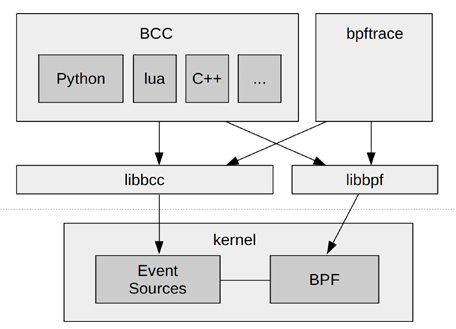
\includegraphics{obrazky-figures/bcc.png}
    }
  \caption{BCC, bpftrace, and BPF \cite{BPFPerformanceTools}.}
  \label{pic:bcc}
\end{figure}

\subsection*{extended Berkeley Packet Filter - eBPF}
Rozšířený Berkeley Packet Filter\cite{EBpf} povoluje spouštět programy v rámci operačního systému a přidávat další funkce za běhu.
eBPF se používá pro  poskytování vysoce výkonných sítí a vyvažování zátěže v moderních datových centrech a cloudových nativních prostředích,
získávání podrobných dat o pozorovatelnosti zabezpečení při nízké režii, pomáhá vývojářům aplikací sledovat aplikace,
poskytování přehledů pro řešení problémů s výkonem a mnoho dalšího.

\subsection*{Funkce}

Přehled základních funkcí, které BPF nabízí.

\subsubsection*{Bezpečnost}

Pochopení všech systémových volání s kombinací na všechny síťové operace přínáší nové přístupy k zabezpečení systému. Pomocí BPF kontrolovat trasování, kontrolu a viditelnost za účelem tvorby bezpečnějších systémů fungujicí na větším úrovní kontroly.

\subsubsection*{Sledování síťového provozu}

BPF poskytuje rozhranní k datové lince, což umožňuje odesílání a přijímání paketů spojové vrstvy. BPF podporuje filtrování paketů a umožňuje \hyperref[sec:UzivatelskeProcesy]{uživatelským procesům},
aby si samy vyfiltrovaly pakety, které chtějí obdržet a které naopak zahodit. Toto může vést ke zvýšení výkonu operačního systému, protože se tím zamezí kopírování nepotřebných paketů.

\subsubsection*{Sledování a profilování}

Možnost připojovat BPF programy ke \hyperref[sec:SledovaciBod]{sledovacím bodům} a bodům jádra, umožňuje bezprecedentní sledování samostatnéhé systému a běhového chování aplikací. Díky schopnosti pohledu na systém a aplikaci, lze sledovat výkon systému. Tyto pohledy je možné i kombinovat pro ještě lepší pohled. Pokročilé provedení umožňuje extrahování pouze slysluplných dat místo exportovaní obrovského množství dat, jak to u podobných systémů bývá provedeno.

\begin{figure}[ht]
  \centering
  \scalebox{1.04}{
        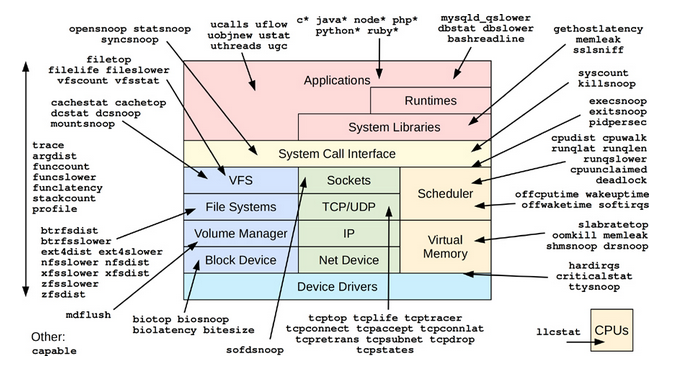
\includegraphics{obrazky-figures/observable.png}
    }
  \caption{Přehled sledovatelných systémových částí \cite{BPFPerformanceTools}.}
  \label{pic:observable}
\end{figure}

\iffalse
\subsection*{libbpf}

Libbpf je knihovna, která obsahuje základní
spoleha na typove informace BTF(ODKAZ) CO-RE




https://github.com/libbpf/libbpf

https://www.kernel.org/doc/html/latest/networking/filter.html
\fi

\subsection{bpftool}
\label{sec:bpftool}

Bpftool\cite{bpftool} se využívá ke spravování BPF programů. Tento program obsahuje sadu podprogramů, které zajíšťují generování kódu pro BPF programy, správu a manipulaci BPF prográmů, tvorbu BPF iterátorů, nahrávání prgramů do jádra a mnoho dalšího.

\subsection*{Zobrazení BPF objektů}
Tento příkaz ukáže všechny BPF objekty načtené v systému.
\begin{lstlisting}[language=bash]
    $ bpftool prog list
\end{lstlisting}

\noindent Ukázka možného výstupu:
\begin{lstlisting}[language=bash]
3: cgroup_device  tag 47dd357395126b0c  gpl
	loaded_at 2022-04-19T11:53:08+0200  uid 0
	xlated 504B  jited 309B  memlock 4096B
4: cgroup_skb  tag 6deef7357e7b4530  gpl
	loaded_at 2022-04-19T11:53:08+0200  uid 0
	xlated 64B  jited 54B  memlock 4096B
5: cgroup_skb  tag 6deef7357e7b4530  gpl
	loaded_at 2022-04-19T11:53:08+0200  uid 0
	xlated 64B  jited 54B  memlock 4096B
6: cgroup_device  tag b73cbcf8b8c71a5b  gpl
	loaded_at 2022-04-19T11:53:08+0200  uid 0
	xlated 496B  jited 307B  memlock 4096B
7: cgroup_skb  tag 6deef7357e7b4530  gpl
	loaded_at 2022-04-19T11:53:08+0200  uid 0
	xlated 64B  jited 54B  memlock 4096B
8: cgroup_skb  tag 6deef7357e7b4530  gpl
	loaded_at 2022-04-19T11:53:08+0200  uid 0
	xlated 64B  jited 54B  memlock 4096B
9: cgroup_device  tag ee0e253c78993a24  gpl
	loaded_at 2022-04-19T11:53:09+0200  uid 0
	xlated 416B  jited 255B  memlock 4096B
\end{lstlisting}

\subsection*{Generování souboru}
Tento příkaz přečte soubor \hyperref[sec:vmlinux]{vmlinux} a vygeneruje hlavičkový soubor vmlinux.h, který obsahuje typové definice, které jádro používá.
\begin{lstlisting}[language=bash]
    $ bpftool btf dump file /sys/kernel/btf/vmlinux format c > vmlinux.h
\end{lstlisting}

\subsection{Netem}

Netem\cite{Netem} je softwarový nástroj pomocí které lze vykonávat síťovou emulaci. Síťovou emulaci lze využít k omezení internetových zdrojů
pro měřenou aplikaci pro lepší testování. Netem umí simulovat zpomalení, ztrátu, poškození nebo duplikaci paketů a případně změnu pořadí
paketů. Netem je řízen pomocí nástroje \emph{tc}, který se ovládá pomocí příkazové řádky. Jeho aktuální distribuce je multiplatformě podporována.

\subsection*{Zpoždění paketů}
Tento příkaz přidá zpoždění všech paketů o 100 milisekund. Toto nastavení je ještě omezeno rozlišením jádra.
\begin{lstlisting}[language=bash]
    $ tc qdisc add dev <interface> root netem delay 100ms
\end{lstlisting}

\noindent Lze i nastavit zpoždění pomocí rozdělení. Příklad s normalním rozdělením:
\begin{lstlisting}[language=bash]
    $ tc qdisc change dev <interface> root netem delay 100ms 20ms distribution normal
\end{lstlisting}

\subsection*{Ztráta paketů}
Tento příkaz zajistí ztrátu paketů. 1 paket z 1000 je zahozen. Nejnižší možná nastavitelná hodnota je 0.0000000232\%.
\begin{lstlisting}[language=bash]
    $ tc qdisc change dev <interface> root netem loss 0.1%
\end{lstlisting}

\subsection*{Duplikace paketů}
Příkaz pro duplikaci paketů je podobný jako příkaz pro ztrátu paketů.
\begin{lstlisting}[language=bash]
    $ tc qdisc change dev <interface> root netem duplicate 1%
\end{lstlisting}

\subsection*{Poškození paketů}
Tímto příkazem lze nastavit poškození paketů. Ten zavede bitovou chybu v náhodném offsetu v paketu.
\begin{lstlisting}[language=bash]
    $ tc qdisc change dev <interface> root netem corrupt 0.1%
\end{lstlisting}

\subsection*{Přeuspořádání paketů}
Existují dva způsoby jak nastavit přeuspořádání paketů.
První způsob je pomocí metody gap, která používá přednastavenou sekvekci a změní pořadí každého Ntého paketu.
\begin{lstlisting}[language=bash]
    $ tc qdisc change dev <interface> root netem gap 5 delay 10ms
\end{lstlisting}
Druhá metoda je reorder způsobí, že určité procento paketů se špatně seřadí.
\begin{lstlisting}[language=bash]
    $ tc qdisc change dev <interface> root netem delay 10ms reorder 25% 50%
\end{lstlisting}

\subsection*{Obnovení rozhranní}
Tento příkaz smaže všechno nastavení na rozhranní. Rozhranní bude poté fungovat jako by na něm žádné nastavení nebylo.
\begin{lstlisting}[language=bash]
    sudo tc qdisc del dev <interface> root
\end{lstlisting}



\chapter{Fungování operačního systému Linux}
\label{sec:FungovaniOperacnihoSystemuLinux}

Aby bylo možné s operačním systémem linux pracovat je potřeba vědět jak vlastně celý systém funguje. Při tvorbě běžných aplikací není potřeba
znát operační systém linux nějak dokonale. Ovšem pokud aplikace pracuje v \hyperref[sec:ProstorJadra]{prostoru jádra}, je nutností vědět jak linuxový operační
systém funguje a poté vyhodnotit zda aplikace nemůže nějakým způsobem poškodit tento systém. Aplikace, které jakkoliv pracují v prostou
jádra musí být spuštěny s příkazem \hyperref[sec:SuperUzivatel]{sudo}. Tímto způsobem aplikace získá možnost pracovat v prostoru jádra bez
omezení. Tato kapitola se věnuje základnímu přehledu o fungování linuxu, z jakých částí se skládá a jak s ním lze pracovat.

\section{Vrsty linuxového systému}

Linuxový systém se skládá ze tři hlavních úrovní. Tyto úrovně jsou vyzobrazeny na obrázku \hyperref[pic:StrukturaLinuxu]{níže} současně s jejich komponenty ze kterých se skládají.
Jak je již zmíněno výše, tak aplikace mohou pracovat v uživatelském prostoru nebo v prostoru jádra.

\begin{figure}[ht]
  \centering
  \scalebox{0.81}{
        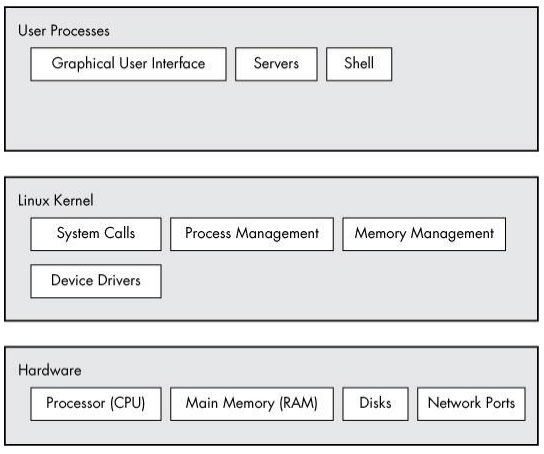
\includegraphics{obrazky-figures/linux_structure.png}
    }
  \caption{Obecná organizace systému Linux \cite{HowLinuxWorks}.}
  \label{pic:StrukturaLinuxu}
\end{figure}

\subsection{Hardware}
Hardware tvoří základ každé výpočetní jednotky. Zahrnuje pamět, jeden nebo více jednotek procesorů pro práci s pamětí. Dále obsahuje hlavní disk a nebo síťového rozhranní. Tato úroveň je nejnižší z těchto tří
úrovní.

\subsection{Linuxové jádro}
\label{sec:ProstorJadra}

Prostřední úrovní je linuxové jádro\cite{HowLinuxWorks}, které je zároveň jádro operačního systému. Jádro je umístěné v paměti, která se také naývá prostor jádra
(angl. kernel space)\cite{KernelSpace}. Je zde uložen a vykonávám kód jádra, který taktéž řídí procesor a říká mu co má dělat.
Jádro především funguje jako rozhranní mezi hardwarem a jakýkoliv spuštěným programem. Zároveň také jádro spravuje hardware.

\subsection{Uživatelské procesy}
\label{sec:UzivatelskeProcesy}

Běžící programy, které jádro spravuje, tvoří nejvyšší úroveň systému. Je také nazýván jako uživatelský prostor.
Uživatelský prostor(angl. user space)\cite{UserSpace} je sada míst, kde běží uživatelské procesy(všechno ostatní kromě jádra). Jádro řídí aplikace v tomto
prostoru tak, aby se nepletly mezi sebou. Procesy, které běží v uživatelském prostoru mají omezenou část paměti a také nemají přístup do
prostoru jádra. Procesy běžící v uživatelském prostoru mohou přistupovat do prostoru jádra jedině přes rozhranní vystavenné prostorem
jádra - \hyperref[sec:systemoveVolani]{systémové volání}. Pokud proces provede systémové volání, tak se do jádra odešle systémové přerušení
a jádro poté obslouží příslušný proces. Jádro pokračuje ve své práci až po dokončení přerušení.

\subsection*{Rozdíly}
Kód běžící v prostoru jádra má neomezený přístup k hlavní paměti a procesoru. Toto je velice silné, ale zároveň velmi nebezpečné privilegium.
Procesy, které zde běží, mohou snadno havarovat celý systém a tím ho nenávratně poškodit.

Naopak v uživatelském prostoru je přístup do paměti omezený na malou podmnožinu a bezpečné operace v procesoru. Jestliže proces z nějakého
důvodu udělá chybu a havaruje, tak jeho následky jsou omezené a jádro je může vyčistit.

Ovšem proces v uživatelském prostoru může také způsobit poškození. Když bude mít vyšší oprávnění než jiné procesy, tak může třeba přepsat
data uložená na disku. Proto je i toto potřeba, dávat si pozor.

\section{Sledovací bod}
\label{sec:SledovaciBod}

Sledovací bod(angl. tracepoint)\cite{Tracepoints} umístěný ve zdrojovém kódu poskytuje tzv. statický háček pro volání funkce(sondy) poskytnutou za běhu aplikace.
Sledovací bod může být zapnutý, pokud je k němu připojena nějaká sonda nebo vypnutý, jestliže k němu žádná sonda připojená není. Když je
sledovací bod zapnutý, tak volá poskytnutou funkci, pokaždé když je sledovací bod spustěň v kontextu provádění volajícího. Když poskytnutá
funkce ukončí své provádění, tak se vrací k volajícímu(pokračuje z místa sledovacího bodu).

Lze je využít pro sledování systému nebo výkonu.

\section{Sonda jádra}

Sonda jádra umožní dynamicky proniknout do rutin jádra a sbírat informace o ladění a výkonu bez přerušení. Existují dva typy sond. První se nazývá kprobe a druhá  kretprobe. Jak každá z nich funguje je popsáno níže.

\subsection*{Jak kprobe funguje}

Jakmile je registrována kprobe, tak kprobe vytvoří kopii probované instrukce a nahradí první bajty instrukcí přerušení. Když procesor zasáhne instrukci bodu přerušení, tak předá řízení kprobe s adresou struktury a provede přidanou funkci. Poté co je funkce provedena, tak se pokračuje následující instrukcí za bodem sondy. Kprobes mohou sondovat běžící jádro, a tím i změnit sadu registrů a ukazatel instrukce. Proto operace s nimi vyžaduje maximální pozornost a znalosti počítačové architektury.

\subsection*{Jak kretprobe funguje}

Při registraci kretprobe se vytvoří kprobe u vstupu do funkce a uloží kopii zpáteční adresy. Nakonec ještě nahradí zpáteční adresu skokem na uživatelsky specifikovaný kus kódu. Jakmile je provedena instrukce návratu, tak se vyvolá sonda a spustí uživatelsky specifikovaný přidaný kus kódu.

\subsection{Optimalizace}

Pokud je jádro sestavené s příznakem \emph{CONFIG\_OPTPROBES=y} a parametr \emph{debug.kprobes\_optimization} je nastaven na 1, tak se pokusí použít instrukce skoku místo instrukcí přerušení pro každou sondu jádra a tím snížit režii probe-hit. Před pokusem o tuto optimalizaci se vloží obyčejná sonda založené na přerušení, takže když se nepovede vložit optimalizovanou verzi sondy, tak tam sonda stále bude.

\subsection{Kontrola bezpečnosti}

Než se provede optimalizace a přidání sondy do jádra, tak se vykoná kontrola bezpečnosti. Kontrola zkontroluje zda oblast, která bude nahrazena instrukcí skoku, leží v rámci jedné funkce(Instrukce skoku má více bajtů, proto může překrývat více instrukcí.). Dále analyzuje celou funkci a ověří konkrétně:

\begin{itemize}[noitemsep]
    \item{funkce neobsahuje žádný nepřímý skok}
    \item{funkce neobsahuje, žádnou instrukci, která by mohla vyvolat výjimku}
    \item{neexistuje žádný skok do optimalizované části}
\end{itemize}

\iffalse
\subsection*{Černá listina}
\subsection*{Rozdíly}

Kernel Probes (Kprobes)
https://docs.kernel.org/trace/kprobes.html
\fi



\section{Sledování událostí}
\label{sec:SledovaniUdalosti}

Sledovací body lze využít ke připojení funkce k určité události\cite{EventTracing} bez vytváření vlastních modulů. Ne všechny sledovací body lze sledovat pomocí systému sledování událostí. K některým musí vývojář poskytnout část kódu, které definují, jaké informace mají být sledovány a případně ukládány.

\subsection*{Formát}
Každý trasovatelná událost má soubor \emph{format}, který obsahuje popis každého pole dané události. Tyto informace lze poté využít v další
analýze. Dále také zobrazuje formátovací řetězec pro tisk události v textovém režimu, název události a ID pro profilování.

Pole v souboru \emph{format} má tvar:
\emph{field:field-type field-name; offset:N;velikost:N;}
Offset je posun pole v záznamu trasování a velikost je velikost dané datové položky určená v bajtech.

\begin{figure}[H]
Příklad události(systémové volání) openat:
\begin{verbatim}
name: sys_enter_openat
ID: 623
format:
    field:unsigned short common_type;	offset:0;	size:2;	signed:0;
    field:unsigned char common_flags;	offset:2;	size:1;	signed:0;
    field:unsigned char common_preempt_count;	offset:3;	size:1;signed:0;
    field:int common_pid;	offset:4;	size:4;	signed:1;

    field:int __syscall_nr;	offset:8;	size:4;	signed:1;
    field:int dfd;	offset:16;	size:8;	signed:0;
    field:const char * filename;	offset:24;	size:8;	signed:0;
    field:int flags;	offset:32;	size:8;	signed:0;
    field:umode_t mode;	offset:40;	size:8;	signed:0;

print fmt: "dfd: 0x%08lx, filename: 0x%08lx, flags: 0x%08lx, mode:
0x%08lx", ((unsigned long)(REC->dfd)), ((unsigned long)(REC->filename)),
((unsigned long)(REC->flags)), ((unsigned long)(REC->mode))
\end{verbatim}
\end{figure}

\subsection*{Spouštěče událostí}

Sledované události jsou vyvolávány spouštěči, které jsou připojeny k daným událostem. Spouštěče mohou být jednoduché příkazy v příkazové řádce či aplikace. Kdykoliv je vyvolána sledovaná událost, která má připojený nějaký spušteč, tak se spustí sada příkazů přidružených k dané události. Ke spouštěči může být navíc připojen filtr. Daná sada příkazů bude spustěna pouze pokud projde daným filtrem. Pokud nemá žádný filtr, tak projde vždy.

K jedné sledované události může být připojen libovolný počet spouštěčů, s výhradou omezení, které mohou mít jednotlivé příkazy.

Spuštěče událostí jsou implementovány v tzv. "měkkém" režimu. Toto zapříčiní, že jakmile je k trasované události připojeno jeden nebo více spouštěčů, tak se aktivuje, i když vlastně není povolen, ale je zakázán v "měkkém" režimu. To znamená, že \hyperref[sec:SledovaciBod]{sledovací bod} bude zavolán, ale nebude sledován, pokud to není skutečně povoleno. Tímto schématem lze vyvolávat spoštěče pro události, které nejsou povoleny, a také umožní použít aktualní implementace filtru událostí při podmíněném vyvolávání spouštěčů.

\section{Systémové volání}
\label{sec:systemoveVolani}

V moderních operačních systémech poskytuje jádro sadu rozhraní, pomocí kterého procesy běžící v uživatelském prostoru můžou interagovat
se systémem. Tato rozhranní poskytují aplikacím přístup k hardwaru, což je mechanismus, díky kterému se dají vytvářet nové procesy,
komunikova se stávájícími a vyžádat si další zdroje od operačního systému. Existence těchto rozhranní a faktem, že aplikace si nemohou přímo
dělat co chtějí, je klíč ke stabilnímu systému.

Systémové volání\cite{LinuxKernelDevelopment} jsou typicky přístupné přes funkce v C knihovně a mají předem definované chování. Mají nula
a více argumentů a můžou mít i návratové hodnoty. Obvykle v datovém typu \emph{long}. Nula je většinou značení pro uspěch a záporná hodnota značí chybu.
Pokud systémové volání vrátí chybu, tak vloží speciální chybnou hodnoru do globalní proměné zvané \emph{errno}. Hodnotu lze přeložit do
lidsky čitelné podoby pomocí funkce \emph{perror()}. Každé systémové volání má konvenci pojmenování, že začíná s \emph{sys\_}.

\subsection*{Komunikace s jádrem}

Systémové volání představují vrstvu mezi hardwarem a uživatelskými procesy. Tato vrsta je primárně pro tři účely.

První účel poskytuje
abstraktní hardwarovou vrstu pro uživatelský prostor. Když aplikace zapisuje nebo čte z disku, tak neví s jakým diskem vlastně pracuje
nebo jaký je souborový systém na kterém je soubor uložen.

Druhý účel je na poskytnutí stability a zabezpečení. Tento účel zabraňuje, aby
aplikace nesprávně používali hardware, nebraly zdroje jiným aplikacím či nepřistupovali k souborům ke kterým nemají povolení.

Poslední účel umožnuje zpracovávat poskytnutý virtualizovaný systém. Kdyby aplikace měly možnost přistupovat ke systémovým zdrojům jak se jim zachce,
tak by bylo nemožné zpracovávat více procesů současně nebo zajistit stabilitu a bezpečnost operačního systému. V linuxových operačních
systémech jsou systémové volání jediný legální vstupní bod k jádru pro uživatelské procesy.

\section{BPF mapy}
\label{sec:BpfMapy}

Technika předávání zpráv k vyvolání chování v programu se široce používá s softwarovém inženýrství. Program může změnit chování jiného programu odesíláním zpráv. Toto také umožňuje výměnu informací a zajištění komunikace mezi těmito programy. Fascinující aspekt BPF je, že kód běžící v jádře a program, který načetl uvedený kód(běží v \hyperref[sec:UzivatelskeProcesy]{uživatelském prostoru}), mohou spolu komunikovat pomocí předávání zpráv.

BPF mapy\cite{LinuxObservabilityWithBpf} ukládají klíče a hodnoty v jádře. Jakýkoliv \hyperref[sec:BPF]{BPF} program k nim může přistupovat, pokud o nich ví. Programy, které běží v \hyperref[sec:UzivatelskeProcesy]{uživatelském prostoru}, mohou také přistupovat k těmto mapám pomocí deskriptorů souboru. Do map lze uložit jakýkoliv druh dat, pokud je předem známá jejich velikost. Jádro používá klíče a hodnoty jako binární bloby a nezajímá se o to, co je zde uloženo.

Verifikátor \hyperref[sec:BPF]{BPF} obsahuje zabezpečení, které zajistí, bezpečný způsob vytváření mapy a přístup k ní. Toto je pak zaručeno vždy, když se přistupuje k datům.

\bigskip
Mapa\cite{BpfMaps} je definována:
\begin{itemize}[noitemsep]
    \item{typem}
    \item{maximálním počtem elementů}
    \item{velikostí klíče v bytech}
    \item{velikostí hodnoty v bytech}
\end{itemize}

\begin{lstlisting}[style=c++,caption={Ukázka mapy v jazyce C},captionpos=b]
struct {
    __uint(type, BPF_MAP_TYPE_ARRAY);
    __uint(max_entries, 10);
    __type(value, u16);
    __type(key, u32);
} ports SEC("maps");
\end{lstlisting}

Při definici mapy tímto způsobem se používá makro, které se nazývá atribut sekce \emph{SEC("maps")}. Toto makro řekne jádru, že tato struktura je \hyperref[sec:BPF]{BPF} a podle toho musí být vytvořena.

\subsection{Typy map}

Dokumentace linuxu definuje mapy jako generické datové struktury, do kterých lze ukládat různé datové typy. V průběhu let se vytvořilo mnoho specializovaných datových struktur, které jsou efektivnější při specifických případech použití.

\bigskip
Seznam hlavních struktur, které lze využít při práci s \hyperref[sec:BPF]{BPF}:
\begin{itemize}[noitemsep]
    \item{HASH}
    \item{ARRAY}
    \item{PERF EVENT ARRAY}
    \item{QUEUE}
    \item{STACK}
\end{itemize}

\iffalse
popsat ringbuffer, ktery neni datova struktura = popsat, slozitost
https://www.kernel.org/doc/html/latest/bpf/ringbuf.html
\fi


\section{BTF formát}

BTF\cite{BTF} je formát pro metadata, který zakóduje informace o ladění související s programem \hyperref[sec:BPF]{BPF}. Původně byl používán k popisu datových typů, ale byl rozšířen, aby zahrnoval další informace. Využívá se pro tisk \hyperref[sec:BpfMapy]{map}, podpisu funkcí, atd. Informace o řádcích pomáhají generovat zdrojový bajtový kód.

BTF specifikace obsahuje dvě části:

\quad \quad - BTF jádrové aplikační rozhranní

\quad \quad - BTF ELF souborový formát

Jádrové aplikační rozhranní je rozhranní mezi uživatelským prostorem a jádrem. Jádro si samo zkontroluje informace o BTF než informace použije.

ELF souborový formát je smlouva uživatelského prostoru mezi souborem ELF a zavaděčem programu \hyperref[sec:BPF]{libbpf}.

\section{Systémový soubor vmlinux}
\label{sec:vmlinux}

Vmlinux soubor obsahuje celé zkompilované nekompresované jádro operačního systému a je uložen ve složce \emph{/sys/kernel/btf/vmlinux}. Existuje i soubor vmlinuz, který se liší tím, že je komprimovaný.

Pomocí tohoto souboru lze díky nástroji \hyperref[sec:bpftool]{bpftool} vygenerovat hlavičkový soubor vmlinux.h, který je vygenerovaný z instalovaného jádra. Soubor obsahuje všechny typové definice, které jádro využívá. Tento hlavičkový soubor se využívá ke kompilování \hyperref[sec:BPF]{BPF} programů jako je to znázorněné na obrázku \hyperref[pic:PostupKompilaceBPF]{níže}. Konkrétně je zahrnut do kompilování kódu pro jádro.

\begin{figure}[H]
  \centering
  \scalebox{0.59}{
        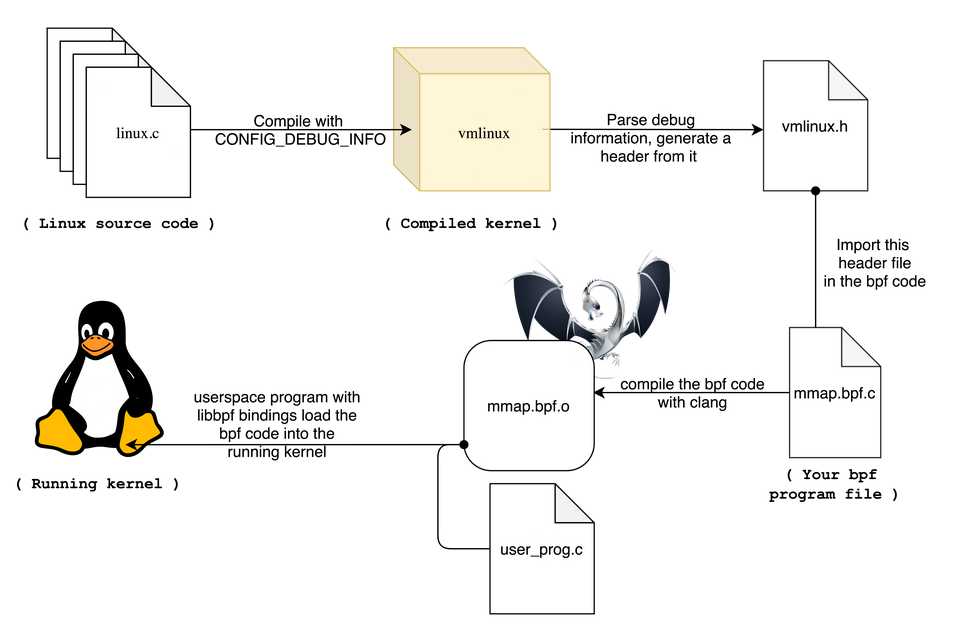
\includegraphics{obrazky-figures/vmlinux.png}
    }
  \caption{Postup kompilace BPF prgramu \cite{}.}
  \label{pic:PostupKompilaceBPF}
\end{figure}

\iffalse
https://lwn.net/Articles/531148/
https://www.csse.uwa.edu.au/programming/linux/Linux-HowTo-9/Kernel-HOWTO/kernel_files_info.html#vmlinuz
najit asi jine zdroje nez tyhle dva
mozna tento
http://www.mnis.fr/fr/services/virtualisation/pdf/LinuxSymposium2004_V1.pdf

citace k obrazku:
https://www.grant.pizza/blog/vmlinux-header/
mozna lepsi pouzit:
https://www.ebpf.top/post/intro_vmlinux_h/
\fi

\section{Superuživatel}
\label{sec:SuperUzivatel}

V linuxových systémech lze spustit příkazy pod superuživatelem\cite{Sudo} nebo jiným uživatelem. Využivá se k zápisu nebo čtení paměti, ke které normalní uživatel nemůže přistupovat. Jako příklad může být přístup do složky \emph{/sys}. Bezpečnostní politika určuje, jaká oprávnění, pokud uživatel nějaká má, musí splnit, aby mohl příkaz spustit. Zásada může vyžadovat ověření uživatelů pomocí hesla nebo jiným autentizačním mechanismem. Zásady zabezpečení podporují ukládání pověření do mezipaměti, aby uživatel mohl spustit sudo bez nutnosti autentizace. Toto nastavení je nastaveno na určitou dobu. Výchozí nastavení je 5 minut. Samotný příkaz sudo lze spustit s přepínači. Pro výpis pomocné zprávy se používá přepínač \emph{h}.

Takové příkazy se provádí pomocí použití slova \emph{sudo} před zadávaný příkaz. Poté se uživatelm musí ověřit autentizačním mechanismem nebo heslem. Jakmile je toto splněno, tak se spustí nová relace v terminálu pod daným uživatelem. Tuto relace lze vypnout pomocí stisknutí kláves \emph{CTRL + C}.

